% テーブルの太線代替(未定義エラー回避)
\newcommand{\thline}{\hline}

\subsubsection{概要}
きなこチームでは,
つくばチャレンジ2025の走行に向けて,
大容量な3次元占有格子地図を実用的に扱うための地図圧縮と,
動的環境での安定走行を目的としたナビゲーションシステムの改良を行った.
本稿では,
ベクトル量子化による3次元占有格子地図の圧縮結果と,
ナビゲーションシステムおよび自己位置推定の拡張内容,
さらにシステム統合について報告する.

\subsubsection{占有格子地図の圧縮}
まず, 占有格子地図の圧縮を行う.
今年のきなこチームの目標に関連して,
ベクトル量子化による3次元占有格子地図の圧縮手法を提案している\cite{船井2026}.
地図はGLIM\cite{glim}\cite{glim_github}を用いて3次元点群地図を作成し,
それを元に占有格子地図を生成した.
その結果,
つくばチャレンジの地図は表\ref{tab:3d_occupancy_grid_map}に示すように
非常に大きい容量となった.
30.9GBの地図は搭載したノートPCの計算機上で他ノードと共存させると
メモリの圧迫, 地図のロード時間増大, 他のプログラムの動作遅延等を招く.
また, Raspberry Pi 4上ですべてのプログラムを動作させることも想定しているため,
メモリ上に展開できないサイズの地図は使用できない.
そこで, ベクトル量子化を用いて地図の圧縮を行った.
圧縮にはvq\_occupancy\_compressor\cite{vq_occupancy_compressor_github}を使用した.

\begin{table}[tb]
  \centering
	\caption{つくばチャレンジ2025環境の3次元占有格子地図}
  \label{tab:3d_occupancy_grid_map}
  \small
	\begin{tabular}{lc}
		\\
    \thline
		地図容量           & 30.9GB \\
    \hline
		実環境における規模 & 795.2$\times$523.6$\times$74.2m \\
    \hline
    解像度             & 0.1m/voxel \\
    \thline
  \end{tabular}
\end{table}

圧縮した結果, \ref{tab:compression_result}に示すように,
地図容量は74.6MBとなり, 圧縮率は0.0024となった.
これは, 搭載する計算機で十分に運用できる容量である.

\begin{table}[tb]
  \centering
	\caption{圧縮結果}
  \label{tab:compression_result}
  \small
	\begin{tabular}{lc}
		\\
    \thline
		圧縮地図の容量 & 74.6MB \\
    \hline
		圧縮率 & 0.0024 \\
    \thline
  \end{tabular}
\end{table}


\subsubsection{開発したナビゲーションシステム}
本チームでは,
自己位置推定にemcl2\_ros2\cite{emcl2_ros2}を,
ナビゲーションには自作したkinako\_nav\cite{kinako_nav_github}を採用した.

当初, navigation2を採用していたが,
つくばチャレンジのような動的障害物や対向ロボットが頻繁に交錯する実環境において, 以下の課題に直面した.
\begin{itemize}
\item 複雑なスタック構成により処理が重くなり, リアルタイムな軌道更新が困難
\item 多数のプラグインとパラメータの相互依存により, 環境に対する最適なチューニングが困難
\item ローカルプランナーの計算窓の制約上, 他のロボットに相当接近してからでなければ回避行動を開始できず衝突のリスクが残存
\item グローバルプランナー, ローカルプランナー, およびリカバリ動作の切り替えロジックが複雑であり, 状況に応じたスムーズなモード遷移が困難
\end{itemize}

これらの課題を解決するため,
Fast Marching Method (FMM) を用いたナビゲーションシステムを開発した.
本システムは,
LiDARの観測範囲全域を単一のポテンシャル場として計算するため,
経路計画と障害物回避を単一の処理系で完結させることが可能となった.
これにより, モード切り替えに伴う判断の遅延やスタックが解消され,
一貫性のある滑らかな挙動になると考えられる.

FMMの計算量は O(NlogN) と極めて効率的であるため,
LiDARが捉えた観測範囲全域の情報をリアルタイムにポテンシャル場へ反映できる.
これにより, 遠方の対向ロボットや障害物を考慮し,
余裕を持った予見的な回避行動を可能にする.

また, 空間の全座標においてゴールへ向かう勾配が定義されているため,
不測の回避行動によって本来の予定進路から外れた場合でも,
瞬時に現在地からの最適ルートを指し示すことができる.

また, 圧縮した3次元地図を利用し, 自己位置推定の信頼性を向上させる目的で,
emcl2\_ros2を拡張した.
具体的には,
圧縮地図の読み出し機能を追加し,
従来2次元スキャンのみ対応していたemcl2\_ros2を3次元点群に対応させた.
ただし,
3次元の自己位置推定は計算量が大きいため,
推定する自由度は2次元(x, y, yaw)に制限した.

さらに,
3D LiDARの点群から高さ領域を指定して抽出し,
走行中に使用する高さを切り替える機能を実装した.
これにより,
人が多く地表付近の点群が遮蔽されやすい場所では地上から離れた高さの点群を使うなど,
場所ごとに特徴的な高さの点群を使い分けられる.

システムの開発のために以下のいくつかのパッケージを作成した.

\begin{itemize}
  \item imu\_rpy\_pose: IMUの角速度を積分し, 位置・姿勢を算出
  \item obstacle\_tracker: スキャンをクラスタリングして障害物マスクを生成
  \item pointcloud2\_cutter: 点群を高さ領域で切り出し, 自己位置推定用の点群と障害物検出用の2次元スキャンを生成
  \item waypoint\_manager: ウェイポイントの管理
  \item vector\_field\_planner: ベクトル場でローカル速度指令を生成するプランナ
  \item velocity\_smoother: 速度指令を平滑化
\end{itemize}

\subsubsection{システム統合}
きなこチームのシステム構成を図\ref{fig:kinako_system}, 図\ref{fig:kinako_nav}に示す.
本研究で用いる自律移動系は, センサ処理, 自己位置推定, 障害物回避, 経路追従をROS 2上で分担する分散システムである.
ノート型PCが主計算機となり, 3D LiDARから点群とIMUの計測結果を取得する.
pointcloud2\_cutterは点群から必要な高さ領域を抽出し,
自己位置推定に用いる点群と障害物検出に用いる2次元スキャンを生成する.
imu\_rpy\_poseは角速度からyawを推定し,
方位の観測としてemcl2\_ros2に与える.
emcl2\_ros2は圧縮地図と点群,
オドメトリを入力とし,
ロボット姿勢を推定する.
waypoint\_followerはmap\_serverから2次元占有格子地図を受信し,
ウェイポイントに基づく目標地点を生成する.
obstacle\_trackerは2次元スキャンをクラスタ化して障害物領域を推定し,
占有領域としてマスクして出力する.
vector\_field\_plannerは地図, 障害物マスク, 目標地点, ロボットの位置を入力として
ロボットの速度指令値を計算する.
最後にvelocity\_smootherが速度を平滑化し, 制御器に送信する.

\begin{figure}[h]
  \begin{center}
    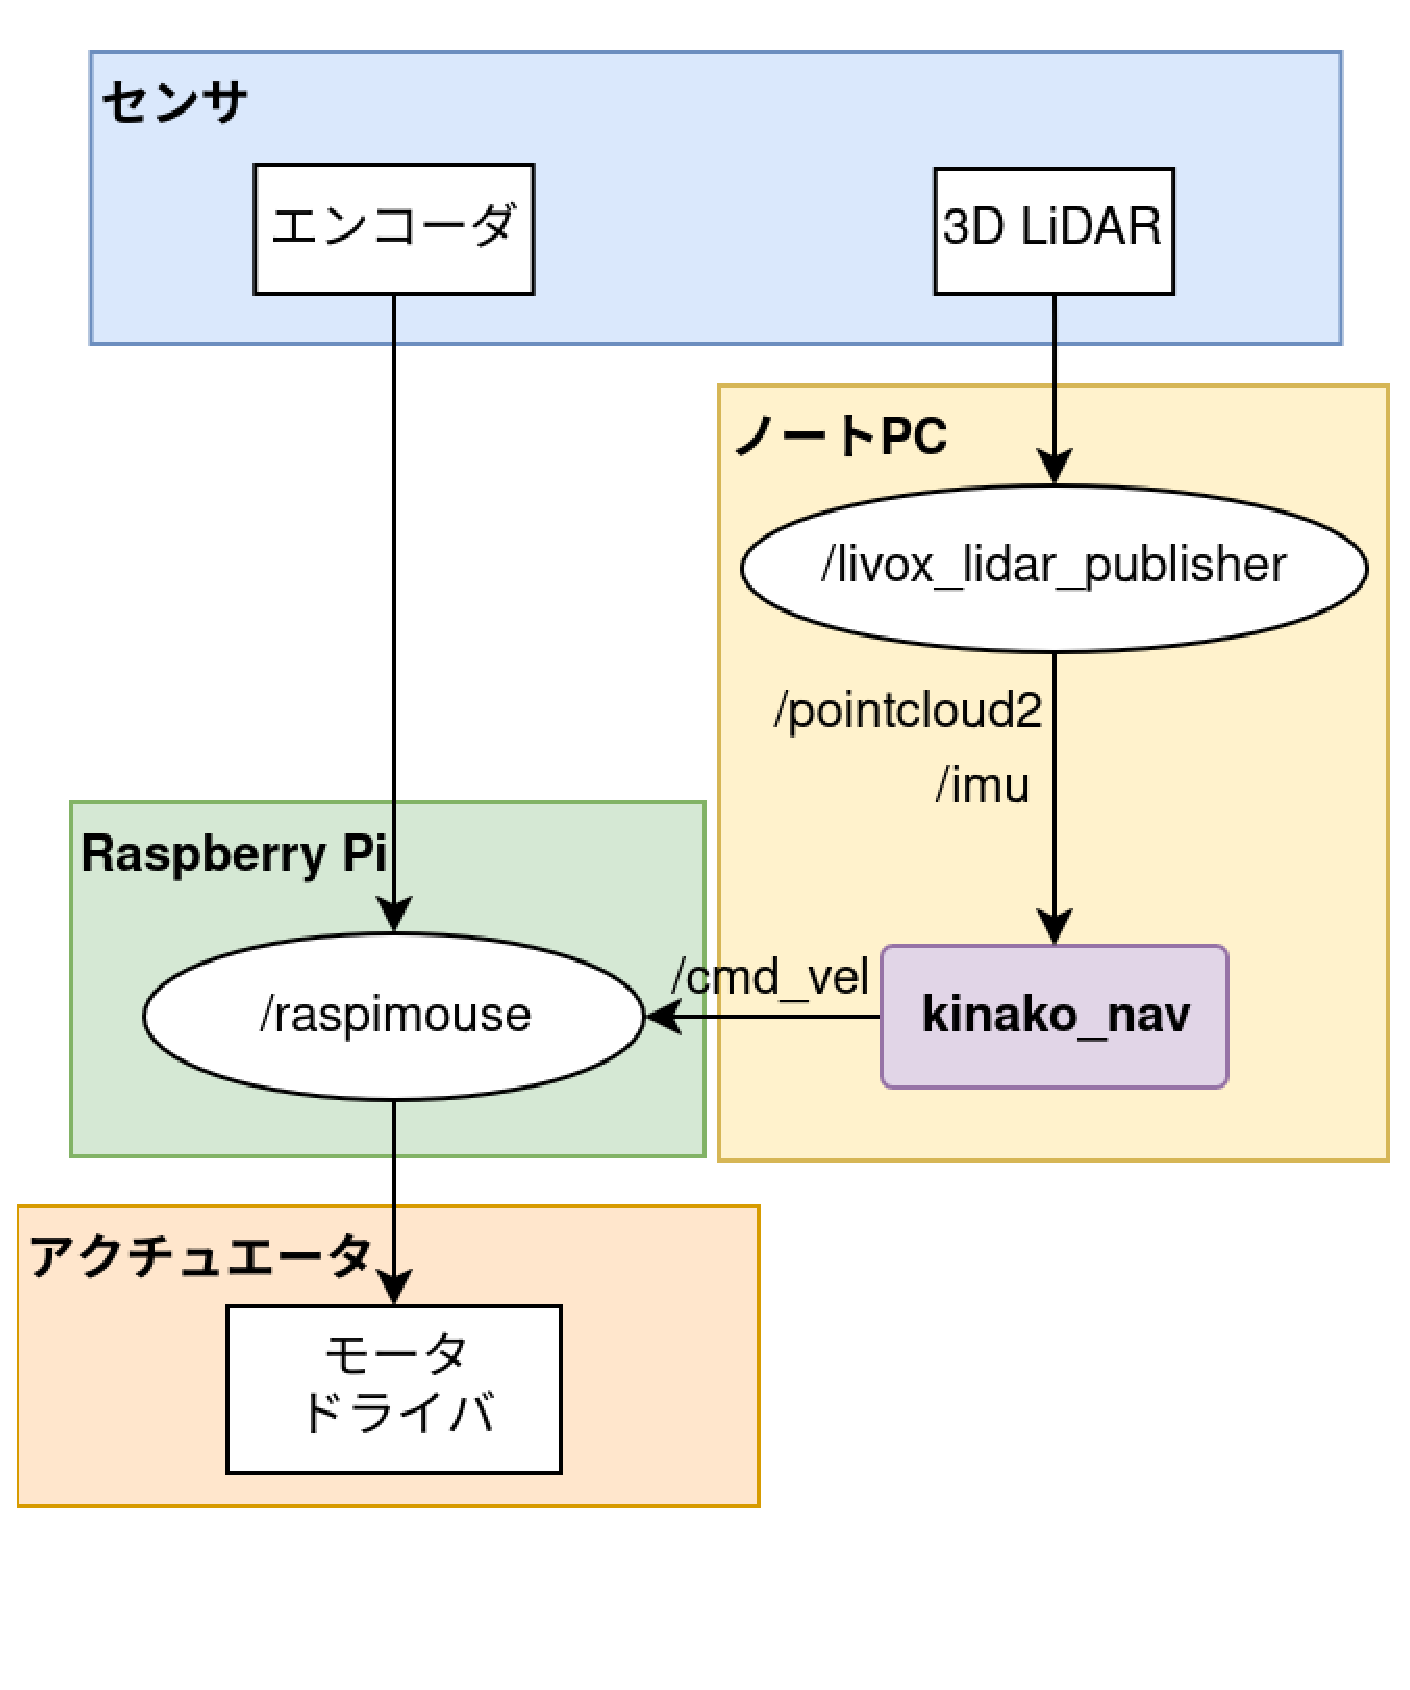
\includegraphics[width=1.0\linewidth]{figs/kinako_system.eps}
    \caption{きなこチームのシステム構成}
    \label{fig:kinako_system}
  \end{center}
\end{figure}

\begin{figure}[h]
  \begin{center}
    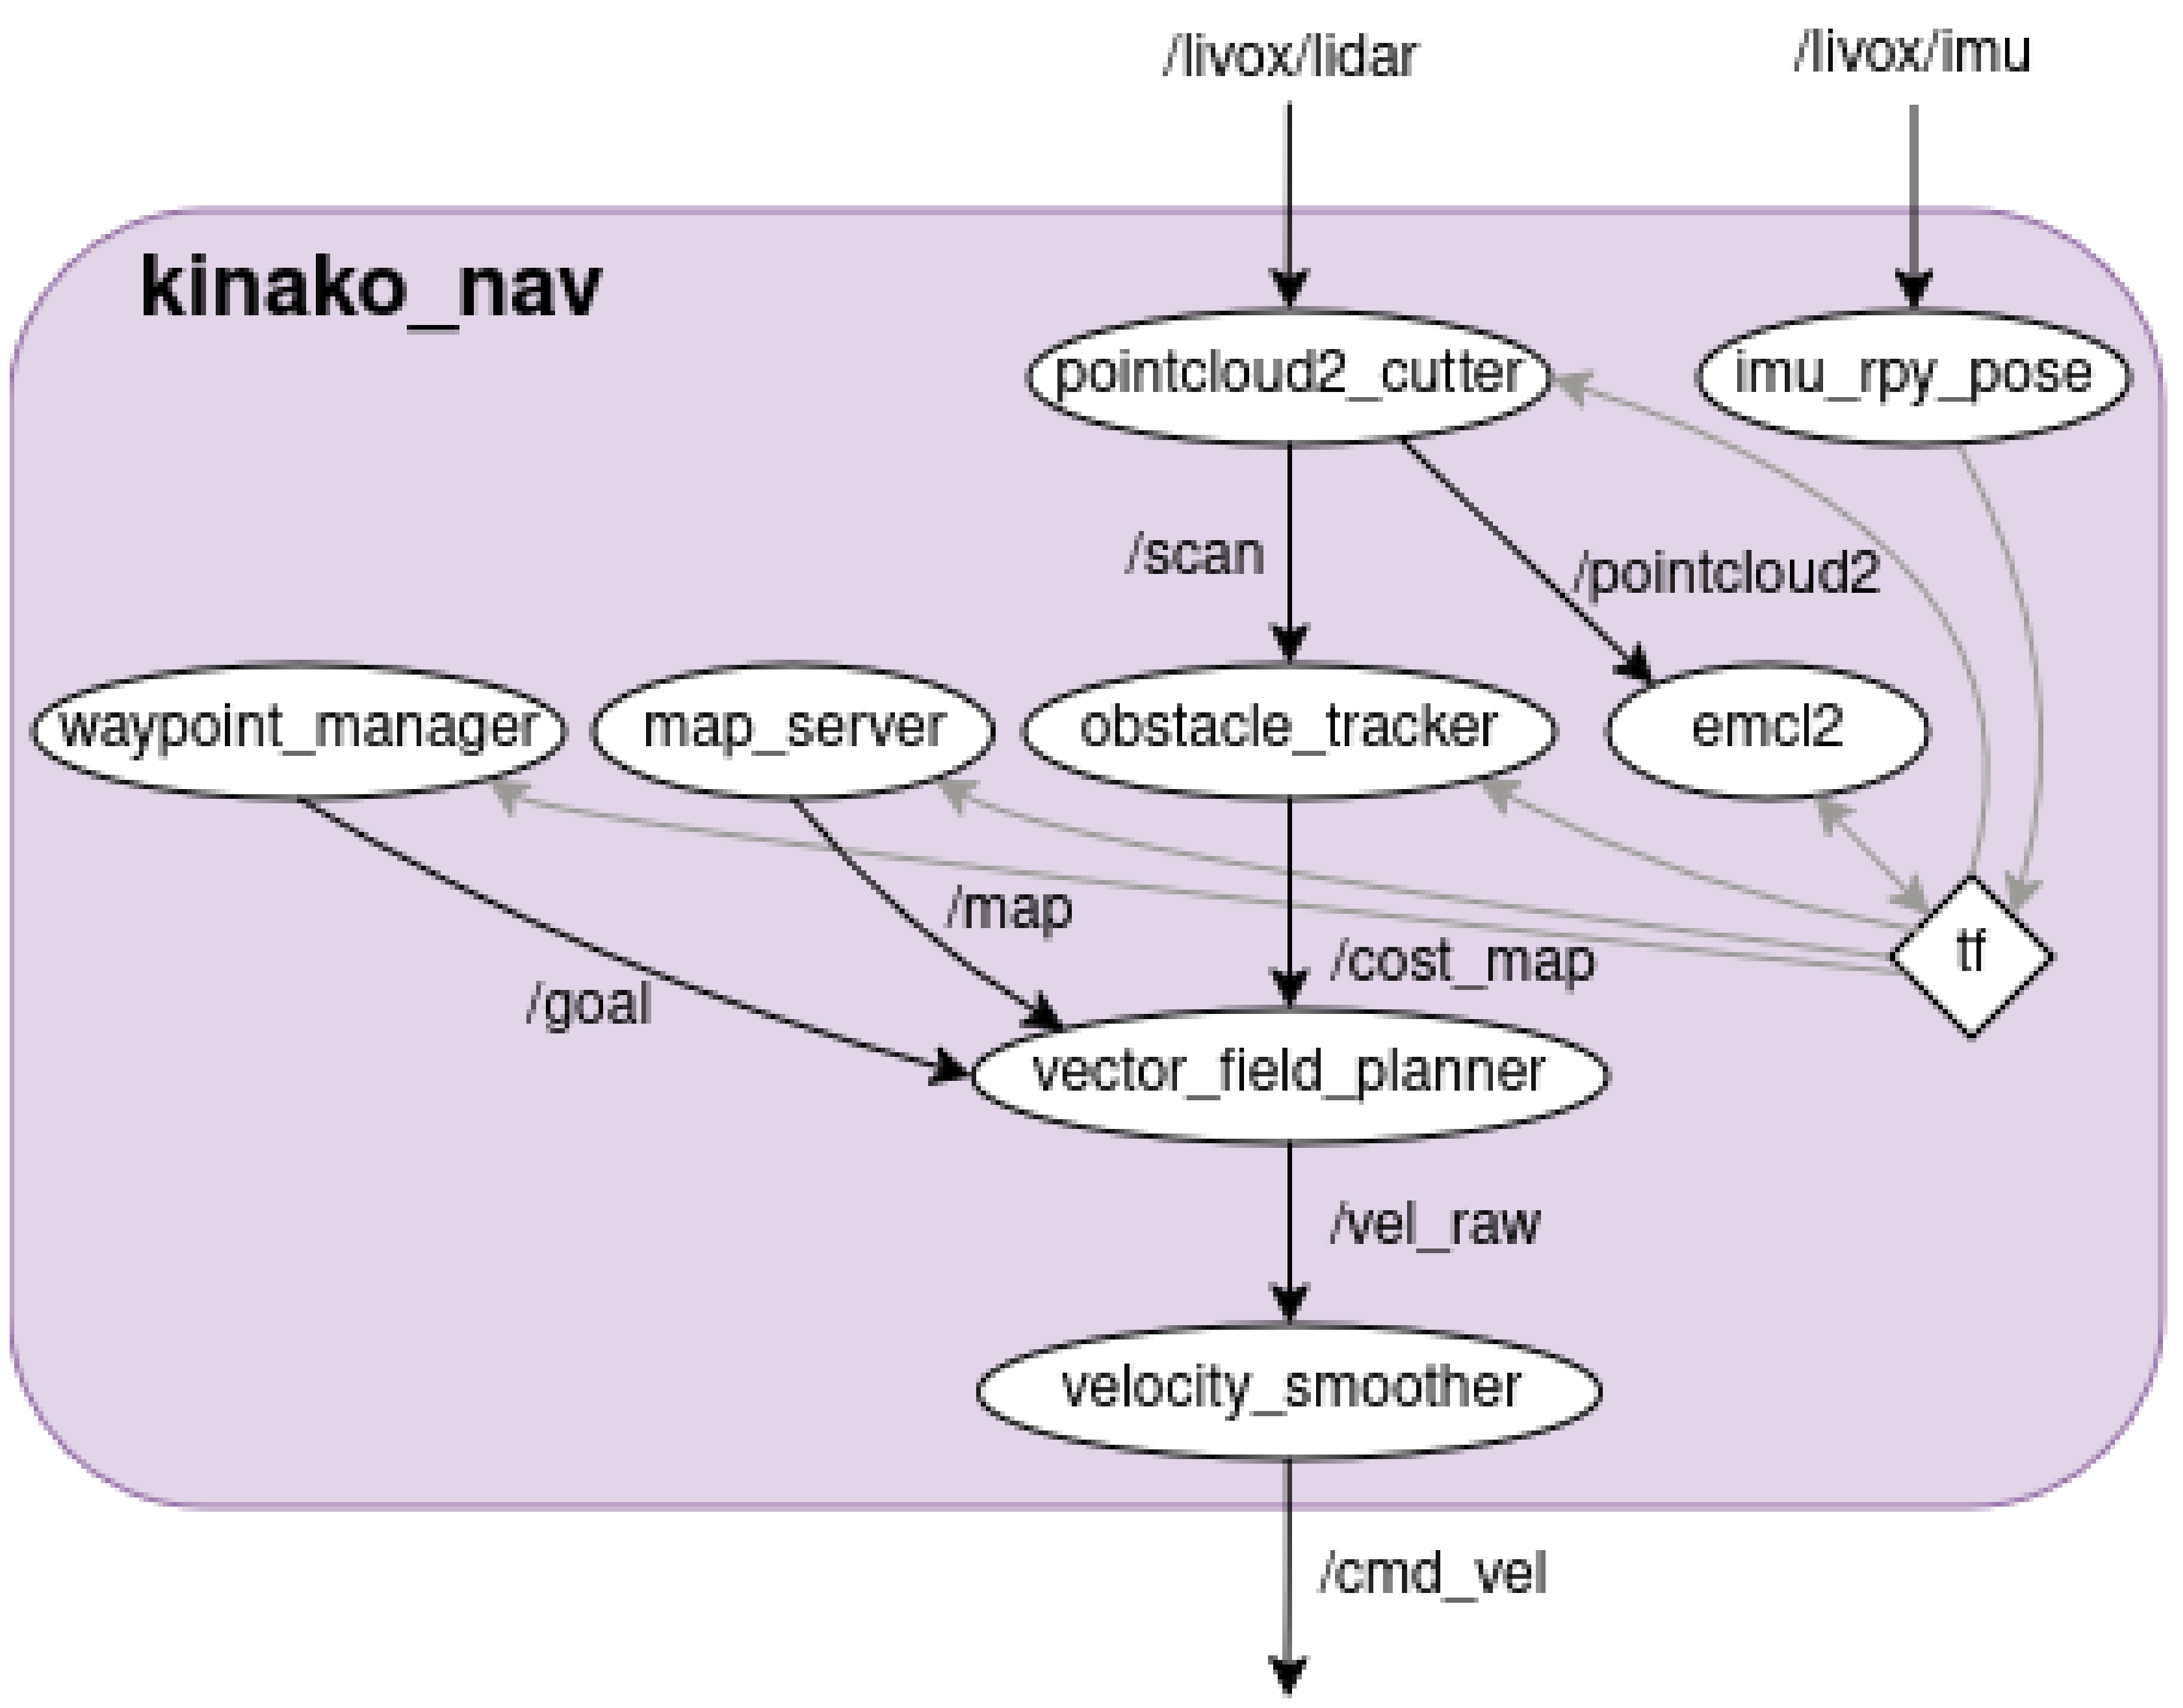
\includegraphics[width=1.0\linewidth]{figs/kinako_nav.eps}
    \caption{kinako\_navのシステム構成}
    \label{fig:kinako_nav}
  \end{center}
\end{figure}
